%% what is the area of the research
% - topic: software development/design/analysis
% - domains: automotive, aeronautics, ..
% - areas: iot, embedded systems, cyber-physical, distributes systems...
% - methods: model-based development, formal methods, ...
% - problems: increasing complexity, stringent standards, market competitiveness, compatibility

An embedded system is some combination of computer hardware and software, either fixed in capability or programmable, placed within a larger system. Industrial machines, automobiles, medical equipment, airplanes, vending machines, as well as mobile devices are all possible locations for an embedded system  \cite{WangJiacun2017RES}. In contrast to traditional software systems, e.g., web applications, desktop applications, embedded systems are usually safety critical, which means their failure to operate properly could cause fatalities and immense properties damage. Moreover, they operate in a rogue environment without interruption for a long time, therefore such systems should be dependable in many ways, for instance, they must be timely and reliable. The hardware platforms on which embedded software programs execute are resource constrained, therefore, efficient software partitioning and deployment is crucial especially in the midst of increasing software applications and their increasing functional complexity. In fact, the development of safety-critical embedded systems is driven by stringent functional safety requirements from respective industry standards, e.g., ISO 26262  in automotive systems \cite{iso201126262}, MIL-STD-2167/DO-178C in avionics \cite{Wang2016DevelopingDO-178Cb}, IEC 61511 in process engineering \cite{bond2002iec}, etc, in order to ensure the quality of embedded systems, which is required to be enforced at different levels, including system development, maintenance, and operation. For instance, the ISO 26262 standard for automotive systems highly recommends rigorous methods to specify and analyze the systems, by applying \textit{formal methods} at different levels of system development, such as requirements specification, system design and implementation. Formal methods \cite{OreganUndergraduateScience} are mathematical techniques that can help the specification and analysis of system models, with precision and without ambiguity. In particular, in this thesis, we apply \textit{lightweight formal methods} \cite{lightweigh2001,Agerholm1999AMethods}, which tackle the difficulty of applying formal methods by applying partial specification, modeling, and focused analysis of relevant system parts, thereby facilitating their applicability in practice. 
\begin{figure}[h!]
  \centering
  \begin{subfigure}[b]{0.575\linewidth}
  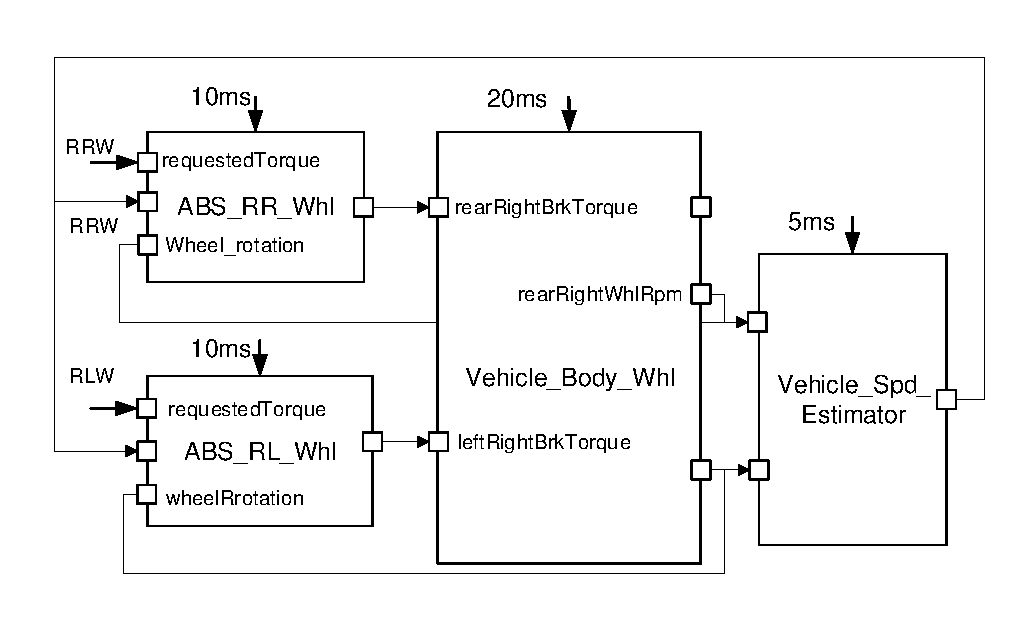
\includegraphics[width=\linewidth]{multirate}
  \caption{Brake-By-Wire Block Diagram.}
     \label{fig_smultirate}
  \end{subfigure}\vspace{-0.05cm}
  \begin{subfigure}[b]{0.4\linewidth}
    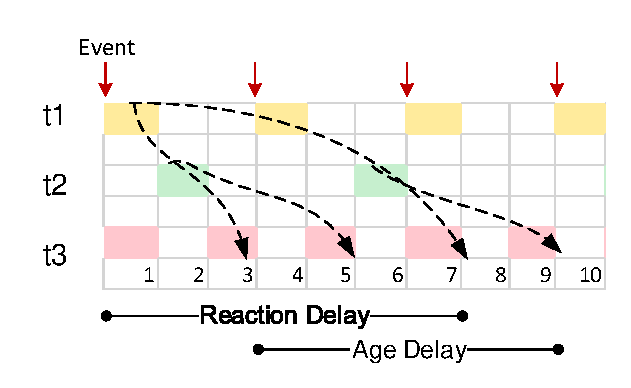
\includegraphics[width=\linewidth]{pics/timedpath.pdf}
    \caption{Timed Paths for the Chain: {\small ABS\_RR\_Whl (t1)$\rightarrow$ Vehile\_Body\_Whl  (t2)$\rightarrow$ Vehile\_Spd\_Estimator  (t3)}.}
    \label{fig_timedpath}
  \end{subfigure}
  \caption{Multirate System, Brake-By-Wire Example.}
  \label{fig_multirate}
\end{figure}

The difficulty of satisfying the timing requirements of embedded systems increases especially when embedded software applications are designed to run over different sampling times (or activation patterns), also known as \textit{multirate}. A multriate design approach enables multitasking by allowing the tasks that realize the functionalities of software applications to execute independently (that is on their own sample time) through interleaving. The timing analysis of multirate systems is complex due the various timed paths that are generated as signals propagate from the sourcing tasks to the sinking tasks. The timed paths are interpreted according to various delay semantics of which the most common are age delay and reaction delay. 
\cite{Feiertag2009ASemantics,mubeen2013support,Becker2017End-to-endSystems}. Multirate designs are widely observed in embedded systems, including in the automotive domain. 

Assuming a Brake-by-Wire (BBW) system that controls the brakes of a car through electrical means, in Figure \ref{fig_smultirate} we show a software application model for the specific part of the BBW system in which the rear-wheel rotation speed and the vehicle speed are used to estimate the target speed, by considering several state and environmental parameters. The \textit{ABS\_RR\_Whl} and \textit{ABS\_RL\_Whl} components are triggered every 10ms to compute the rotational speed of the wheels, which are fed to the \textit{Vehicle\_Body\_Whl} component that runs every 20ms. The \textit{Vehicle\_Spd\_Estimation} component runs every 5ms to compute the target vehicle speed by reading inputs from the previous component and other parameters not shown in the model. Figure \ref{fig_smultirate} shows the timed paths of the age delay (the latest time the signal propagates from input to output) and reaction delay (the earliest time the signal propagates from input to output) of the model. In this thesis, we focus on the design and analysis of multirate embedded systems.

% highlight the problems that you want to address in the thesis
% - requirements specifications: ambiguous, incomprehensible, inconsistencies
% - resource efficiency
% - software design errors, e.g.,  timing errors
\begin{wrapfigure}{R}{0pt}
\centering
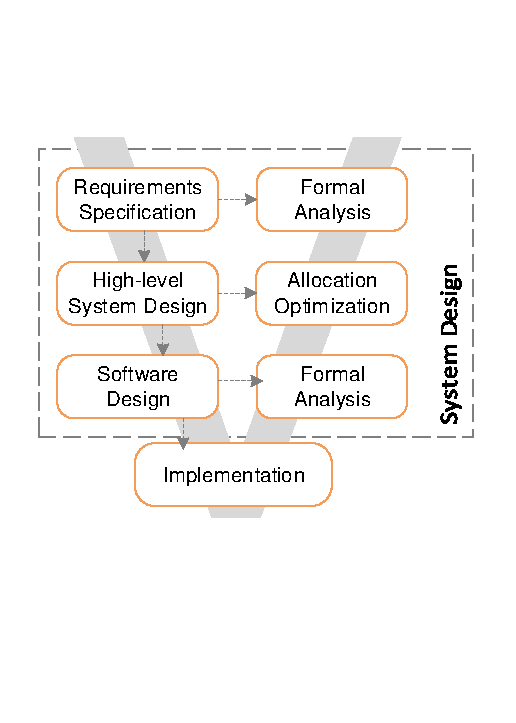
\includegraphics[trim=0 0 0 0,clip,width=0.4\textwidth]{pics/vmodel.pdf}
\caption{\label{fig_vmodel}Top-down Development, in V-model.}
\vspace{-0.4cm}
\end{wrapfigure}
Embedded systems are usually developed over several development stages as illustrated by the V-model in Figure \ref{fig_vmodel}. In the particular case of top-down software development, the requirements specifications are employed in the design of high-level system architecture, as well as in designing the behavior of the software system according to the high-level architecture. In this model of the software development process, the detection and elimination of software errors at early stages is crucial in order to prevent their propagation to the implementation stage. By doing so, the maintenance cost and the time-to-market can be reduced \cite{Ebert2009EmbeddedFuture,Grimm2003SoftwareChallenges}. Therefore, in this thesis, propose scalable and usable ways of applying formal techniques at the requirements specification, system design and software design stages of embedded systems development, in order to assure and thereby improve the quality of embedded systems.

Requirements specifications are structured collections of functional and extra-functional requirements, which are statements that describe the needs that the solution must satisfy \cite{ieereqspecstandard}. The specifications are mainly textual but could also contain diagrams to elaborate the textual representations. The textual representations of requirements are mostly expressed in natural language mainly because natural language is intuitive. Furthermore, natural language is expressive and flexible, so the required system functionality can be sufficiently expressed and communicated easily. However, natural language can be deemed too flexible and unconstrained to the extent that engineers tend to specify requirements that are hard to understand, vague, ambiguous, etc. Template-based methods \cite{Hull2011RequirementsEngineering}, controlled natural language  \cite{attempto96,Schwitter2002EnglishLanguage} and property specification pattern systems with underlaying formal semantics  \cite{Gruhn2006PatternsSpecifications,Konrad2005Real-timePatterns,Post2012AutomotiveBOSCH,Filipovikj2014ReassessingDomain} have been proposed to mitigate most of the natural language drawbacks and misuse. However, due to the lack of effective and scalable methods of specification, the above mentioned problems of requirements specifications persist in practice \cite{Sikora2011RequirementsNeeds}. To address this deficit, we propose a flexible yet structured language, called ReSA [ref], for specifying embedded systems requirements, based on boilerplates and domain-specific concepts. To provide automated support, we also propose the ReSA tool [ref] that also implements a  consistency checking method for system requirements, based on the satisfiability of the Boolean formulas that encode the high-level requirements

At the system design level, the requirements specifications are realized by a system architecture of software and hardware parts that are constructed by functional components (or modules) that abstract the functionality of the system. In the platform-based development approach \cite{Sangiovanni-Vincentelli2004BenefitsDesign}, the system design should take into account consumption of critical hardware resources, such as power consumption, for two main reasons: optimizing power consumption is beneficial in order i) to accommodate more applications as well as to support power-intensive applications, and ii) to increase battery-life by lowering the amount of heat released by electronic components in the system. In this thesis, we propose an exact software allocation approach, as well as a heuristic one, for multirate systems that need to meet both timing and reliability. 

The system architecture is refined further by software design units, whose behavior is often specified in Simulink \cite{JamesB.Dabney2003MasteringSimulink}, which is the de-facto modeling language employed in industry.  To provide assurance that Simulink models fulfill given functional and timing requirements, we propose a pattern-based, execution-order preserving automatic transformation of atomic and composite Simulink blocks into stochastic timed automata that can be formally analyzed with UPPAAL Statistical Model Checker \cite{Bulychev2012UPPAAL-SMC:Automata}. Our method is scalable, and has been validated on industrial use cases \cite{Filipovikj2016SimulinkSystems}. The statistical model checking analyzes a state-transition system by conducting statistical analysis on the collected traces of the system executions, effectively mitigating the state-space explosion of (exact) model checking \cite{Legay2010StatisticalOverview}. 

The rest of the thesis proposal is organized as follows. Section \ref{section:goals} introduces the research goals and the scientific contributions to address the research goals. Section \ref{section:methods} presents the research methods applied to conduct the research especially in the context of academic-industry collaboration. Section \ref{section:outline} shows the proposed outline of the thesis, followed by the presentation of the research progress in Section \ref{section:progress}, including the time plan until the doctoral defense. Section \ref{section:thirdcycle} presents the third-cycle outcomes, adapted from the individual study plan (ISP). Finally, Section \ref{section:related} discusses the related work before concluding the proposal in Section \ref{section:conclusions}.